\documentclass[aspectratio=1610]{beamer}
\usepackage[utf8]{inputenc}
\usepackage[T1]{fontenc}
\usepackage{booktabs}
\usepackage{amsmath}
\usepackage{graphicx}
\usepackage{bbm}

\usepackage[
    natbib=true,
    bibencoding=inputenc,
    bibstyle=authoryear-ibid,
    citestyle=authoryear-comp,
    maxcitenames=3,
    maxbibnames=10,
    useprefix=false,
    sortcites=true,
    backend=biber
]{biblatex}

\title{Specialization Trends in Economics Research\\
using JEL Codes}
\subtitle{Research Proposal Presentation for Topics Course Text Data in Economics}
\date{January 21, 2025}
\author{Felix Schmitz}

\usetheme{UniBonn}

\begin{document}
\usebeamertemplate{custom equation spacing}

\begin{frame}[plain]
	\titlepage
\end{frame}

\begin{framecontent}
	\frametitle{Table of contents}
\end{framecontent}

%%%%%%%%%%%%%%%%%%%%%%%%%%%%%%%%%%%%%%%%%%%%%%%%%%%%%%%%%%%%%%%%%%%%%%%%%%%%%%%%%%%%%%%%%%%%
\section{Motivation}
%%%%%%%%%%%%%%%%%%%%%%%%%%%%%%%%%%%%%%%%%%%%%%%%%%%%%%%%%%%%%%%%%%%%%%%%%%%%%%%%%%%%%%%%%%%%

\begin{frame}
	\frametitle{Motivation}
	\begin{center}
		\bfseries{
			Are subfields in economics research becoming more specialized?\\
			Are there new subfields emerging?\\
			Are Journal of Economic Literature (JEL) codes of publications helpful in answering these questions?
		}
	\end{center}

	To answer these questions, I will:
	\begin{itemize}
		\item Analyze the use of individual JEL codes in economics research over time
		\item Inspect the combinations of JEL codes used (combinations vanishing/emerging)
		\item Compare results to other research methods analyzing specialization trends
	\end{itemize}
\end{frame}

\begin{frame}
	\frametitle{Motivation}
	\framesubtitle{A primer on JEL codes}
	\begin{itemize}
		\item Journal of Economic Literature: quarterly published by the American Economic Association
		\item JEL Codes are a classification system for research articles widely used in Economics
		\item Hierarchical structure with single character and two-digit codes
		\item Self-classification by authors (may be adapted during review process)
		\item Categories range from general economics to specific subfields, but do not cover methods
		\item Example follows
	\end{itemize}
\end{frame}

\begin{frame}
	\frametitle{Motivation}
	\framesubtitle{Example: Galiani (2023) classified as JEL A11, A14}
	\textbf{A. General Economics and Teaching}
    \begin{itemize}
        \item A1 General Economics
        \begin{itemize}
            \item A10 General
            \item \textbf{A11 Role of Economics • Role of Economists • Market for Economists}
            \item A12 Relation of Economics to Other Disciplines
            \item A13 Relation of Economics to Social Values
            \item \textbf{A14 Sociology of Economics}
            \item A19 Other
        \end{itemize}
        \item A2 Economic Education and Teaching of Economics
        \begin{itemize}
            \item A20 General
            \item A21 Pre-college
            \item $\cdots$
        \end{itemize}
        \item A3 Collective Works
        \begin{itemize}
            \item A30 General
            \item $\cdots$
        \end{itemize}
    \end{itemize}
	\textbf{B. History of Economic Thought, Methodology, and Heterodox Approaches}	
\end{frame}

\begin{frame}
	\frametitle{Motivation}
	\framesubtitle{Literature}
	\begin{itemize}
		\item Heikkila (2022): History of JEL codes and potential research applications
		\item Heikkila (2024): Uses abstracts and LLMs to create (artificial) JEL codes for comparison
		\item Kelly (2011): Analyze the publication of subjects, the development of JEL codes, and define specialty journals using JEL codes (1969-2007)
		\item Rath (2016): Build upon the work of Kelly (2011) and analyze general JEL code use developments (add 2007-2013)
		\item Angrist (2017) and Angrist (2020): NLP techniques to assign specific field of economics research tags
		\item Galiani (2023) (first presentation): Used both hand-coded and machine-coded articles to analyze specialization trends in fields of economics research
	\end{itemize}
\end{frame}

%%%%%%%%%%%%%%%%%%%%%%%%%%%%%%%%%%%%%%%%%%%%%%%%%%%%%%%%%%%%%%%%%%%%%%%%%%%%%%%%%%%%%%%%%%%%
\section{Data Sources}
%%%%%%%%%%%%%%%%%%%%%%%%%%%%%%%%%%%%%%%%%%%%%%%%%%%%%%%%%%%%%%%%%%%%%%%%%%%%%%%%%%%%%%%%%%%%

\begin{frame}
	\frametitle{Data Sources}
	\framesubtitle{already acquired}

	\textbf{Constellate}
	\begin{itemize}
		\item Metadata (title, DOI, author names, publication date, journal of publication)
		\item unigrams, bigrams, and trigrams
	\end{itemize}

	\textbf{Semantic Scholar}
	\begin{itemize}
		\item Metadata (title, publication date, identifiers, authors, fields of study tags)
		\item Abstracts
		\item Comprehensive citation and reference data
	\end{itemize}

	\textbf{Galiani (2016) and Galiani (2020)}
	\begin{itemize}
		\item Manually tagged field of economics research
		\item Include: applied, applied theory, econometric methods, theory
	\end{itemize}
\end{frame}

\begin{frame}
	\frametitle{Data Sources}
	\framesubtitle{initial sample}

	\textbf{Research Papers in Economics (RePEc) IDEAS}
	\begin{itemize}
		\item Metadata (title, author, publication date, journal of publication)
		\item JEL codes
		\item Accessible via FTP server (connecting to all publisher FTP servers providing the metadata)
		\item A Python package for accessing RePEc data is available on \href{https://github.com/andrei-dubovik/repec}{GitHub} (not used yet)
	\end{itemize}
\end{frame}

\begin{frame}
	\frametitle{Data Sources}
		\framesubtitle{challenges so far}
	
		\begin{itemize}
			\item \textbf{Data availability:} Open access limited, especially full dataset download
			\begin{itemize}
				\item Constellate will be discontinued in June
				\item Semantic Scholar broader coverage but less detailed metadata
				\item RePEc discourages scraping, no public API, no documentation of dataset building
				\item EconLit (American Economics Association) behind paywall
			\end{itemize}
			\item \textbf{Size of dataset:} 
			\begin{itemize}
				\item APIs are rare, hence datasets contain large number of variables
				\item Constellate and Semantic Scholar sample from Galiani (2023) are 6GB (each) in zipped format
			\end{itemize}
			\item \textbf{Data quality:}
			\begin{itemize}
				\item JEL codes are self-assigned by authors
				\item JEL codes are not always assigned
				\item JEL codes may reflect the content poorly
			\end{itemize}
		\end{itemize}
	\end{frame}

%%%%%%%%%%%%%%%%%%%%%%%%%%%%%%%%%%%%%%%%%%%%%%%%%%%%%%%%%%%%%%%%%%%%%%%%%%%%%%%%%%%%%%%%%%%%
\section{Methodology}
%%%%%%%%%%%%%%%%%%%%%%%%%%%%%%%%%%%%%%%%%%%%%%%%%%%%%%%%%%%%%%%%%%%%%%%%%%%%%%%%%%%%%%%%%%%%

\begin{frame}
	\frametitle{Methodology}
	\begin{itemize}
		\item \textbf{Trends of individual JEL codes used:}
		\begin{itemize}
			\item Publication counts of individual JEL codes over time
			\item Average number of JEL codes per article
			\item Analysis of the above in combination with journals
		\end{itemize}

		\item \textbf{Cluster analysis of JEL code combinations:}
		\begin{itemize}
			\item Clustering of JEL code combinations (e.g. via Louvain method for community detection)
			\item Analysis of clusters over time
		\end{itemize}

		\item \textbf{Comparison to other research methods:}
		\begin{itemize}
			\item Use of text data methods will be highly relevant here
			\item Topic modeling via n-grams, LDA, or available data sources
			\item Comparison to other research fields via Constellate or Semantic Scholar data
		\end{itemize}
	\end{itemize}
\end{frame}

\begin{frame}
	\frametitle{Methodology}
	\framesubtitle{A primer on Louvain method}
	\begin{itemize}
		\item Goal is to find non-overlapping communities inside a large network
		\item Nodes are individual JEL codes, and edges represent the strength of their co-occurrence
		\item Iterative process of optimizing modularity $Q$ via a weighted graph
		\begin{equation}
			Q = \frac{1}{2m} \sum_{i=1}^N \sum_{j=1}^N \left( A_{ij} - \frac{k_i k_j}{2m} \right) \delta(c_i, c_j)
		\end{equation}
		\item $A_{ij}$: edge weight between nodes $i$ and $j$
		\item $k_i$ and $k_j$: sum of weights of edges connected to each nodes $i$ and $j$ 
		\item $m$: sum of all edge weights
		\item $N$ number of nodes
		\item $c_i$ and $c_j$: community assignment of nodes $i$ and $j$
		\item $\delta(c_i, c_j) = \mathbbm{1}[c_i = c_j]$: Kronecker delta function
	\end{itemize}
\end{frame}

\begin{frame}
	\frametitle{Methodology}
	\framesubtitle{A primer on Louvain method (continued)}
	\begin{itemize}
		\item Modularity $Q$ of community $c$ then becomes:
		\begin{equation}
			Q_c = \frac{1}{2m} \sum_{i=1}^N \sum_{j=1}^N  A_{ij} \mathbbm{1}{c_i = c_j = c} - \left(\sum_{i=1}^N \frac{k_i }{2m} \mathbbm{1}{c_i = c} \right)^2
			= \frac{\Sigma_{in}}{2m} - \left(\frac{\Sigma_{tot}}{2m}\right)^2
		\end{equation}
		\item $\Sigma_{in}$: sum of the weights of the edges inside the community
		\item $\Sigma_{tot}$: sum of the weights of the edges connected to nodes in the community (including to nodes outside the community)
		\item Since the method provides non-overlapping communities:
		\begin{equation}
			Q = \sum_{c=1}^N Q_c
		\end{equation}
	\end{itemize}
\end{frame}

%%%%%%%%%%%%%%%%%%%%%%%%%%%%%%%%%%%%%%%%%%%%%%%%%%%%%%%%%%%%%%%%%%%%%%%%%%%%%%%%%%%%%%%%%%%%
\section{Summary \& Discussion}
%%%%%%%%%%%%%%%%%%%%%%%%%%%%%%%%%%%%%%%%%%%%%%%%%%%%%%%%%%%%%%%%%%%%%%%%%%%%%%%%%%%%%%%%%%%%

\begin{frame}
	\frametitle{Summary \& Discussion}
	\begin{itemize}
		\item Research so far focused on text analysis and not on JEL code combinations
		\item Access to JEL codes so far limited, but feasible
		\item Weakness of JEL codes in representing content and correct assignment
		\item Methodology: Louvain method for community detection (use the information of single JEL code for clustering combinations?)
	\end{itemize}
\end{frame}

\begin{frame}
	\frametitle{Summary \& Discussion}
	\framesubtitle{What else?}

	\begin{center}
		\textbf{Any ideas for understanding specialization trends?\\
		Do you have any suggestions for the methodology?\\
		Any other comments or ideas?}
	\end{center}
\end{frame}

\begin{frame}
    \frametitle{A graphical representation of the Louvain method (Wikipedia)}
    \begin{columns}
        \begin{column}{0.33\textwidth}
            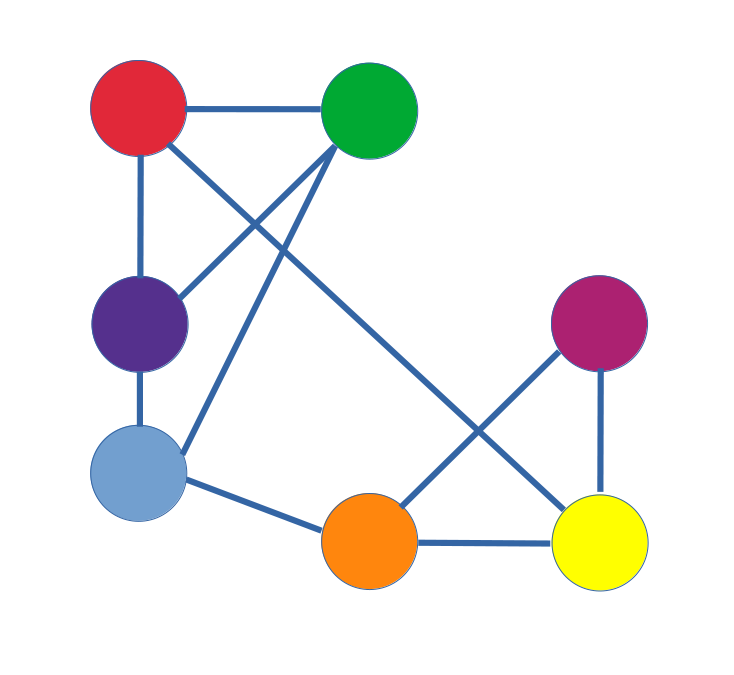
\includegraphics[width=\textwidth]{Louvain_Step1.png}
			\captionof{figure}{Step 1}
			Node initialization with singleton community
        \end{column}

        \begin{column}{0.33\textwidth}
            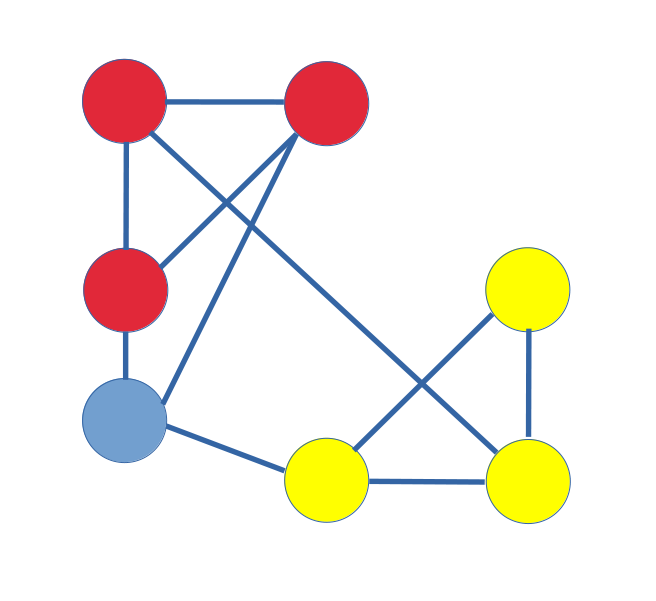
\includegraphics[width=\textwidth]{Louvain_Step2.png}
			\captionof{figure}{Step 2}
			Community assignment based on modularity gain
        \end{column}

        \begin{column}{0.33\textwidth}
            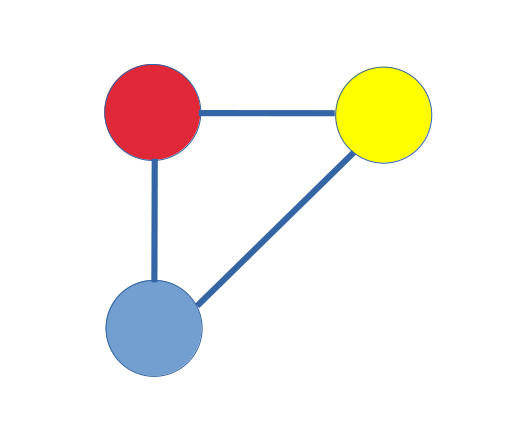
\includegraphics[width=\textwidth]{Louvain_Step3.png}
			\captionof{figure}{Step 3}
			Community aggregation and edge weight update
        \end{column}
    \end{columns}
\end{frame}
\end{document}
